\documentclass{beamer}
 
\usepackage[utf8]{inputenc}
\usepackage[english]{babel}
\usepackage{amsmath}
\usepackage{amsfonts}
\usepackage{amssymb}
\usepackage{graphicx} 
\usepackage{latexsym} 
\usepackage{listings}
\usepackage{xcolor}
\usepackage{soul}
\usepackage[T1]{fontenc}
\usepackage{amsthm}
\usepackage{mathtools}
\usepackage{setspace}
\usepackage{array,multirow,makecell}
\usepackage{geometry}
\usepackage{textcomp}
\usepackage{float}
\usepackage{bbold}
\usepackage{wrapfig}
\usepackage{textpos}

\rmfamily

\usetheme{Madrid}
%%\usecolortheme{beaver}



\title{LC 09 Caractérisations par spectroscopie en synthèse organique}
\author{Naïmo Davier}


 
\begin{document}
	
\begin{frame}
	\titlepage
\end{frame}

\addtocounter{framenumber}{-1}

\title{LC 09 Caractérisations par spectroscopie en synthèse organique}
\institute{Université Paul sabatier}

\begin{frame}

\frametitle{Spectroscopie visible}
\centerline{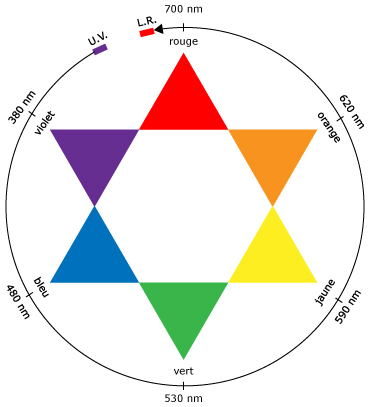
\includegraphics[width=7cm]{couleurs}}
\end{frame}


\begin{frame}
\frametitle{Spectroscopie Infra-rouge}

\centerline{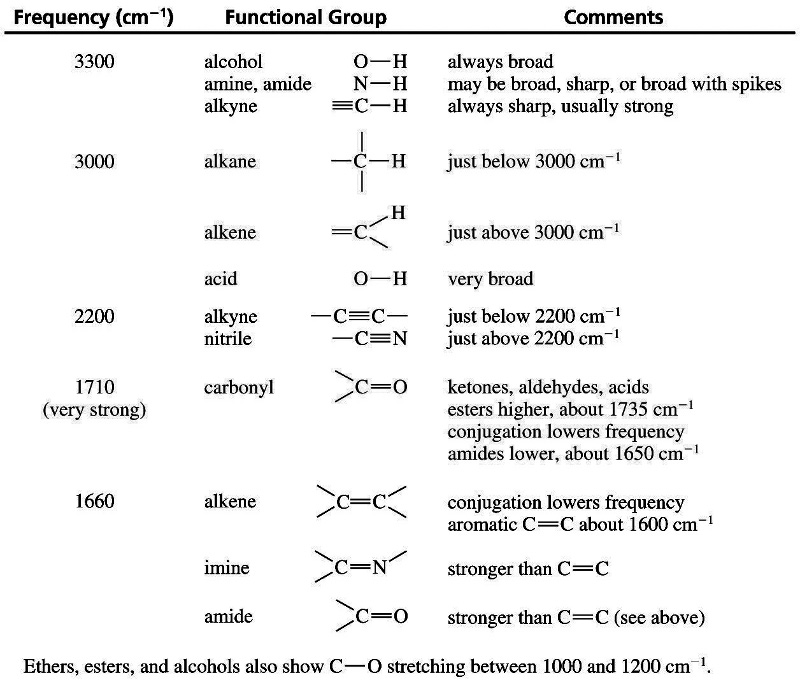
\includegraphics[width=9cm]{IR-Table}}
\end{frame}

\begin{frame}
\frametitle{Spectroscopie Infra-rouge}
\textbf{Synthèse de l'acide benzoïque à partir de l'alcool benzylique}\\
\vspace{0.4cm}
\centerline{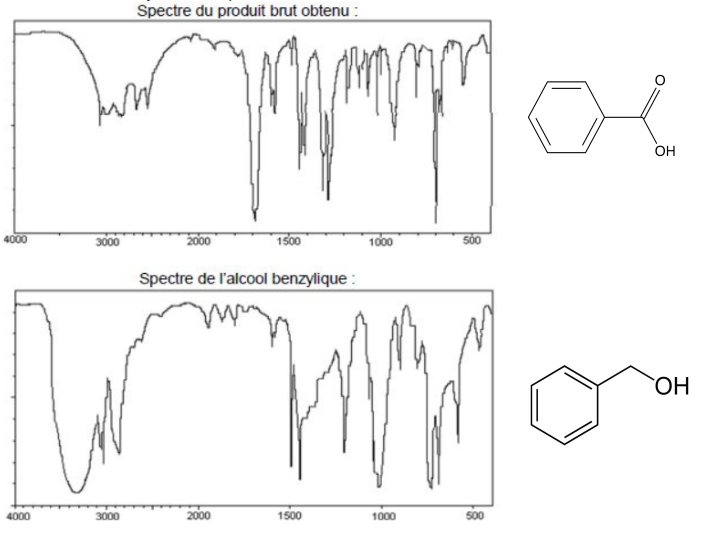
\includegraphics[width=9cm]{spectresIR}}
\end{frame}

\begin{frame}
\frametitle{Spectroscopie RMN}
\textbf{Déplacement chimique et aire : cas du 1-bromo-2,2-diméthylpropane}\\
\vspace{0.4cm}
\centerline{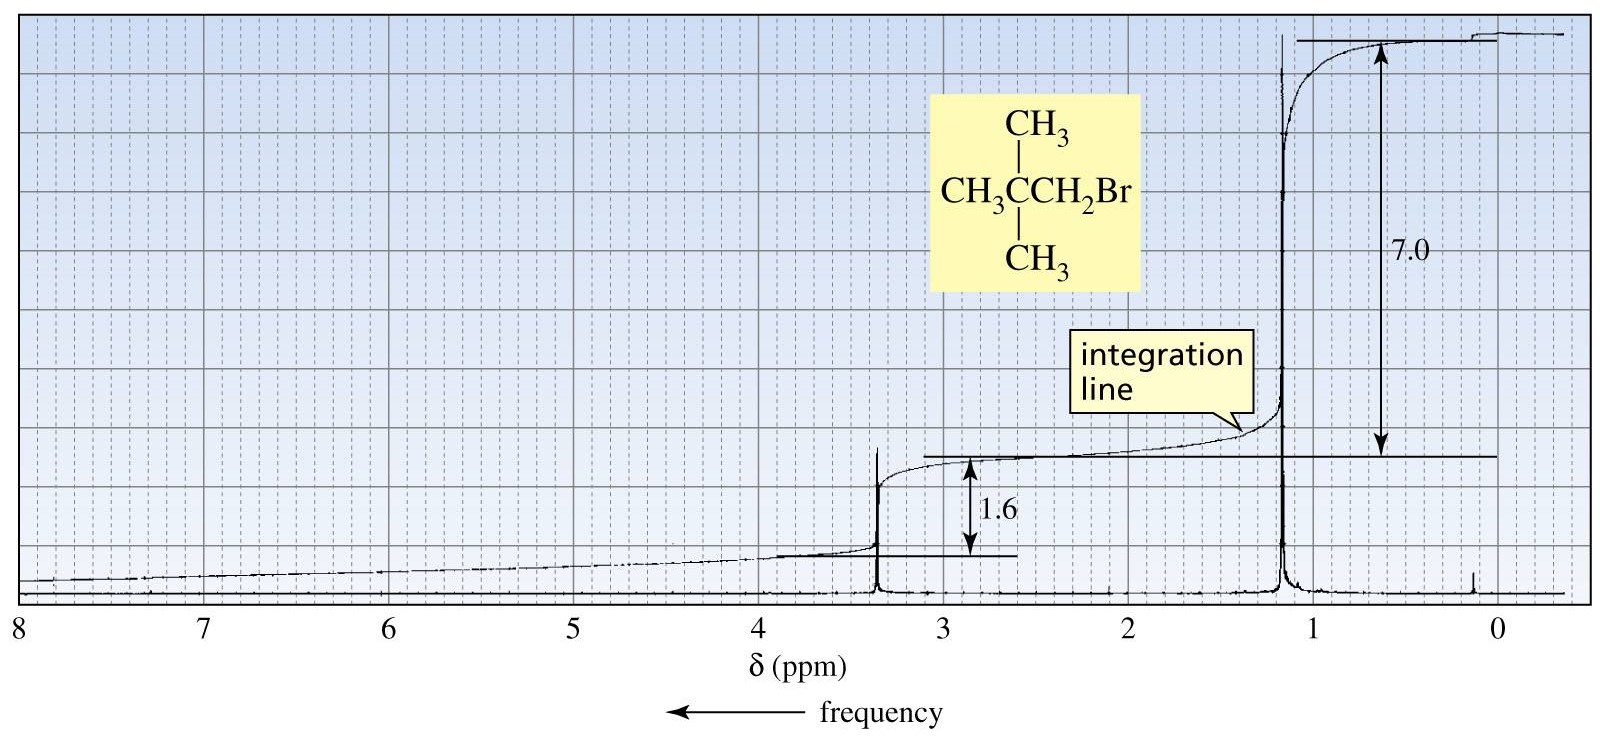
\includegraphics[width=12cm]{spectreRMN1}}
\end{frame}

\begin{frame}
\frametitle{Spectroscopie RMN}
\textbf{Multiplicité : exemple de l'éthanol $CH_3-CH_2-OH$}\\
\vspace{0.3cm}
\centerline{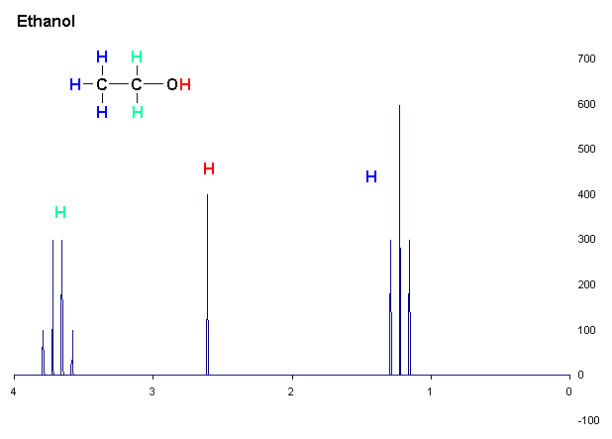
\includegraphics[width=10cm]{RMN2_0}}
\end{frame}

\begin{frame}
\frametitle{Spectroscopie RMN}
\textbf{Application : 4-méthylbenzaldéhyde}\\
\vspace{0.25cm}
\centerline{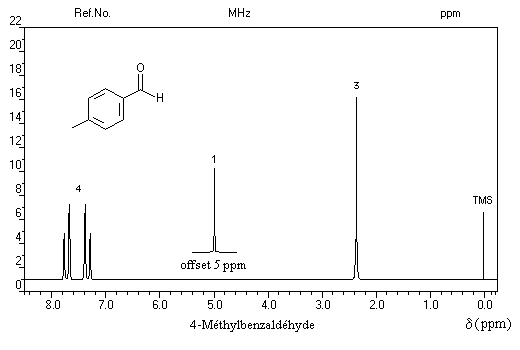
\includegraphics[width=10.5cm]{RMN3}}
\end{frame}

\end{document}